\section{Hardware choices and limitations}\label{sec:hardware}

This section describes the choices made for the project in terms of which hardware is required to construct the \projname{} prototype. In order for the robot to solve the tasks described in \secref{sec:system_definition}, some specific hardware is required. The hardware required for the robot is:

\begin{itemize}
\item Motors to drive and steer the robot.
\item Motors for collecting objects.
\item Sensors to ensure that the robot stays inside the boundaries of the environment.
\item Sensor to detect objects.
\item Sensor for movement precision.
\end{itemize}

There exist a number of available sensors and actuators for the LEGO NXT. These sensors gives the NXT robots the ability to perform various actions. For the required tasks, it has been chosen to use the interactive servo motors for driving, steering, and the collection of objects. The colour sensor is well suited to ensure that the robot can detect the environment boundaries. For detecting objects, the ultrasonic sensor has been chosen, as the robot is required to know when an object is present and should be collected, as well as the distance to the detected object. Finally, to help ensure precise movement, the HiTechnic NXT Compass sensor is used.

\subsection{Hardware test} \label{sec:hardware_test}
In order to know the capabilities and limitations of the hardware, some tests were conducted. Testing environments were set up to test the individual hardware devices. The early data heavy tests \fxnote{"heavy tests" ?} were created in LabView and transferred to the NXT brick. These used the original LEGO NXT firmware. During the test the LEGO Brick would write all the results into a file, which later would be transferred into LabView for analysis. 

Later on, further tests were conducted using the data logging feature in nxtOSEK \citep{datalogging}. A bluetooth connection is established between the NXT brick and a PC, and while the robot is running, the outputs from the sensors and motors are logged and sent to the PC. The data can be saved in a .csv file and converted into graphs, which makes for easy analysis.

\subsubsection{Ultrasonic sensor} \label{sec:ultrasonic_sensor}
The ultrasonic sensor emits an ultrasonic sound wave and measures the time it takes for the wave to impact on an object and return to the sensor. Depending on the time taken, the sensor can measure the distance from the sensor to the detected object~\citep{lego_education}. 

\begin{figure}[H]
     \center{\includegraphics[width=320pt]
     {graphics/DistanceGraph.png}}
     \caption{\label{fig:ultrasonic_sensor_test_graph} The actual distance and the measured distance from the ultrasonic sensor test.}
\end{figure}

The ultrasonic sensor was tested at different distances to measure the accuracy. The test was performed stationary and every 25 ms it sends out a pulse, for 250 seconds, resulting in 1000 pulses, which would give a significant average of the distance. \appref{app:ultrasonic_sensor_test} shows the raw values observed during the test, which has been converted into the graph seen in \figref{fig:ultrasonic_sensor_test_graph}. The graph shows values from the tests from 1 cm to 50 cm. This test was performed using LabView.

\begin{figure}[H]
     \center{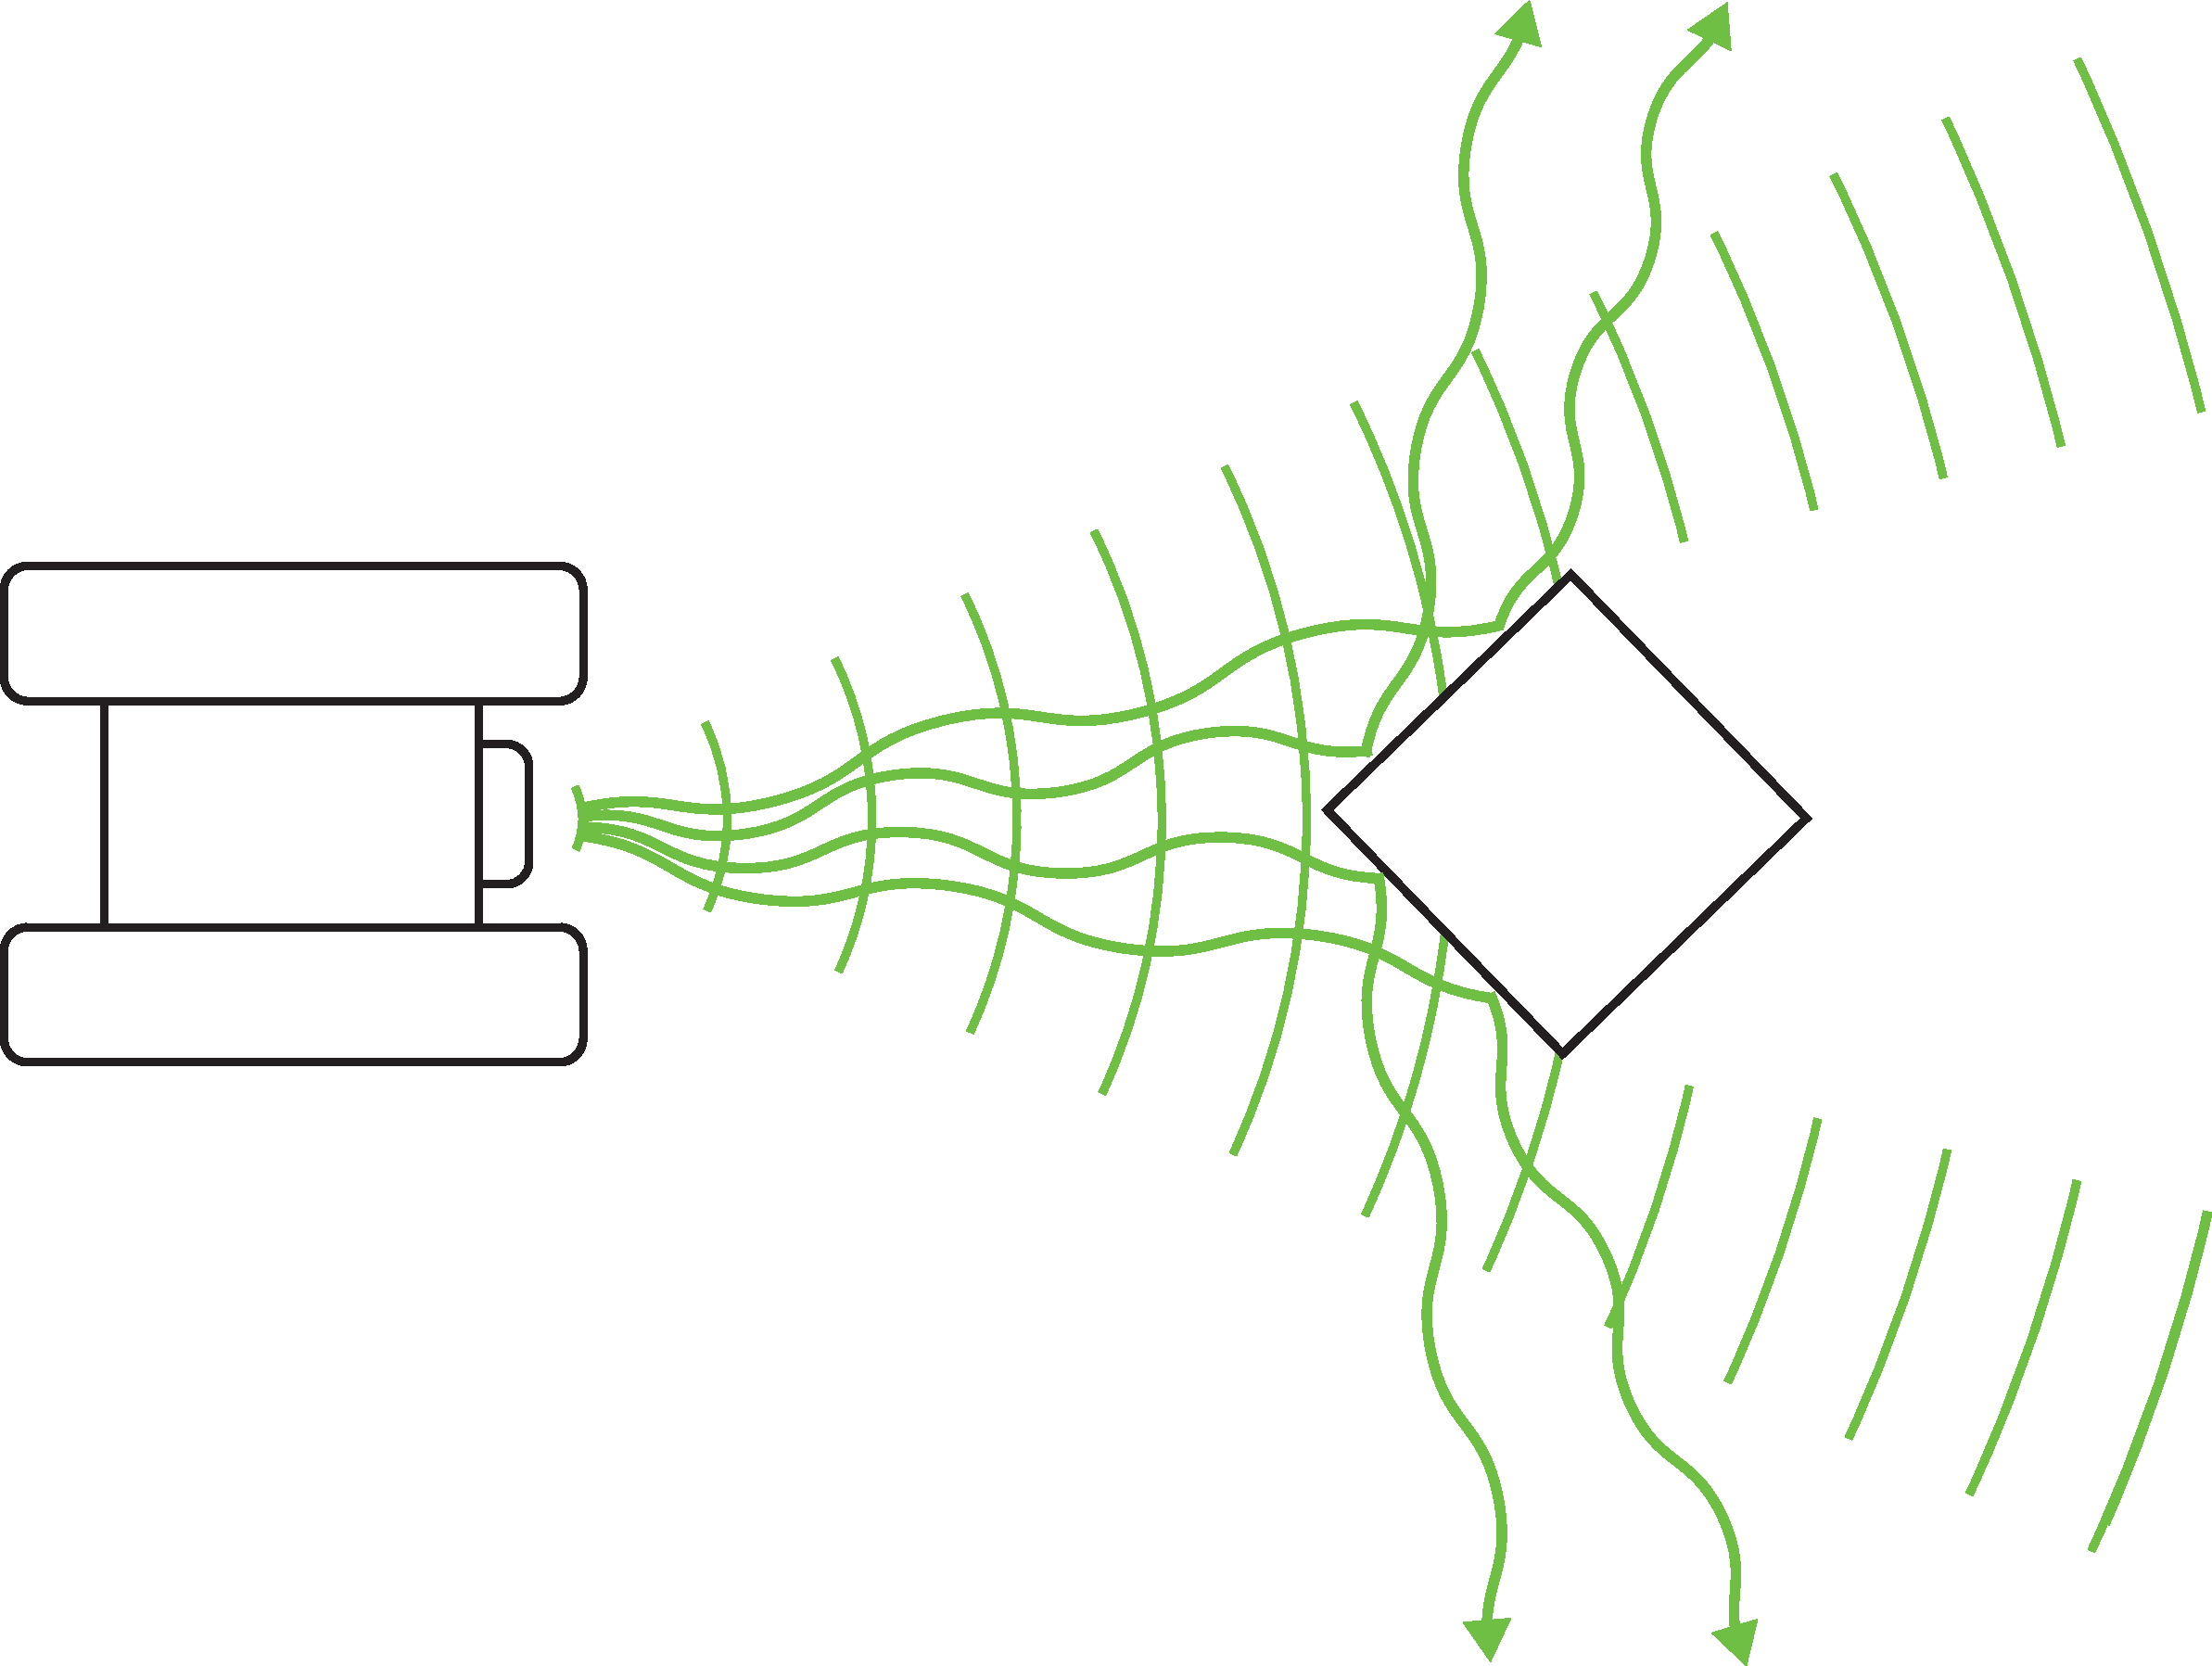
\includegraphics[width=320pt]
     {graphics/SonarWaves.pdf}}
     \caption{\label{fig:angled_object} Sonic waves on an angled object.}
\end{figure}

At short distances, the ultrasonic sensor is proved to be imprecise. This is most highly due to the quality of the sensor and how it is constructed. As the distance increases, the precision increases as well, but does still vary a few cm. The sensor have some problems when it comes to spotting an object at certain angles, for example the angled object illustrated in \figref{fig:angled_object}. The sound waves sent out is reflected away from the sensor. This results in the sensor not being able to correctly calculate the distance and sometimes not being able see the object at all.

\begin{figure}[H]
     \center{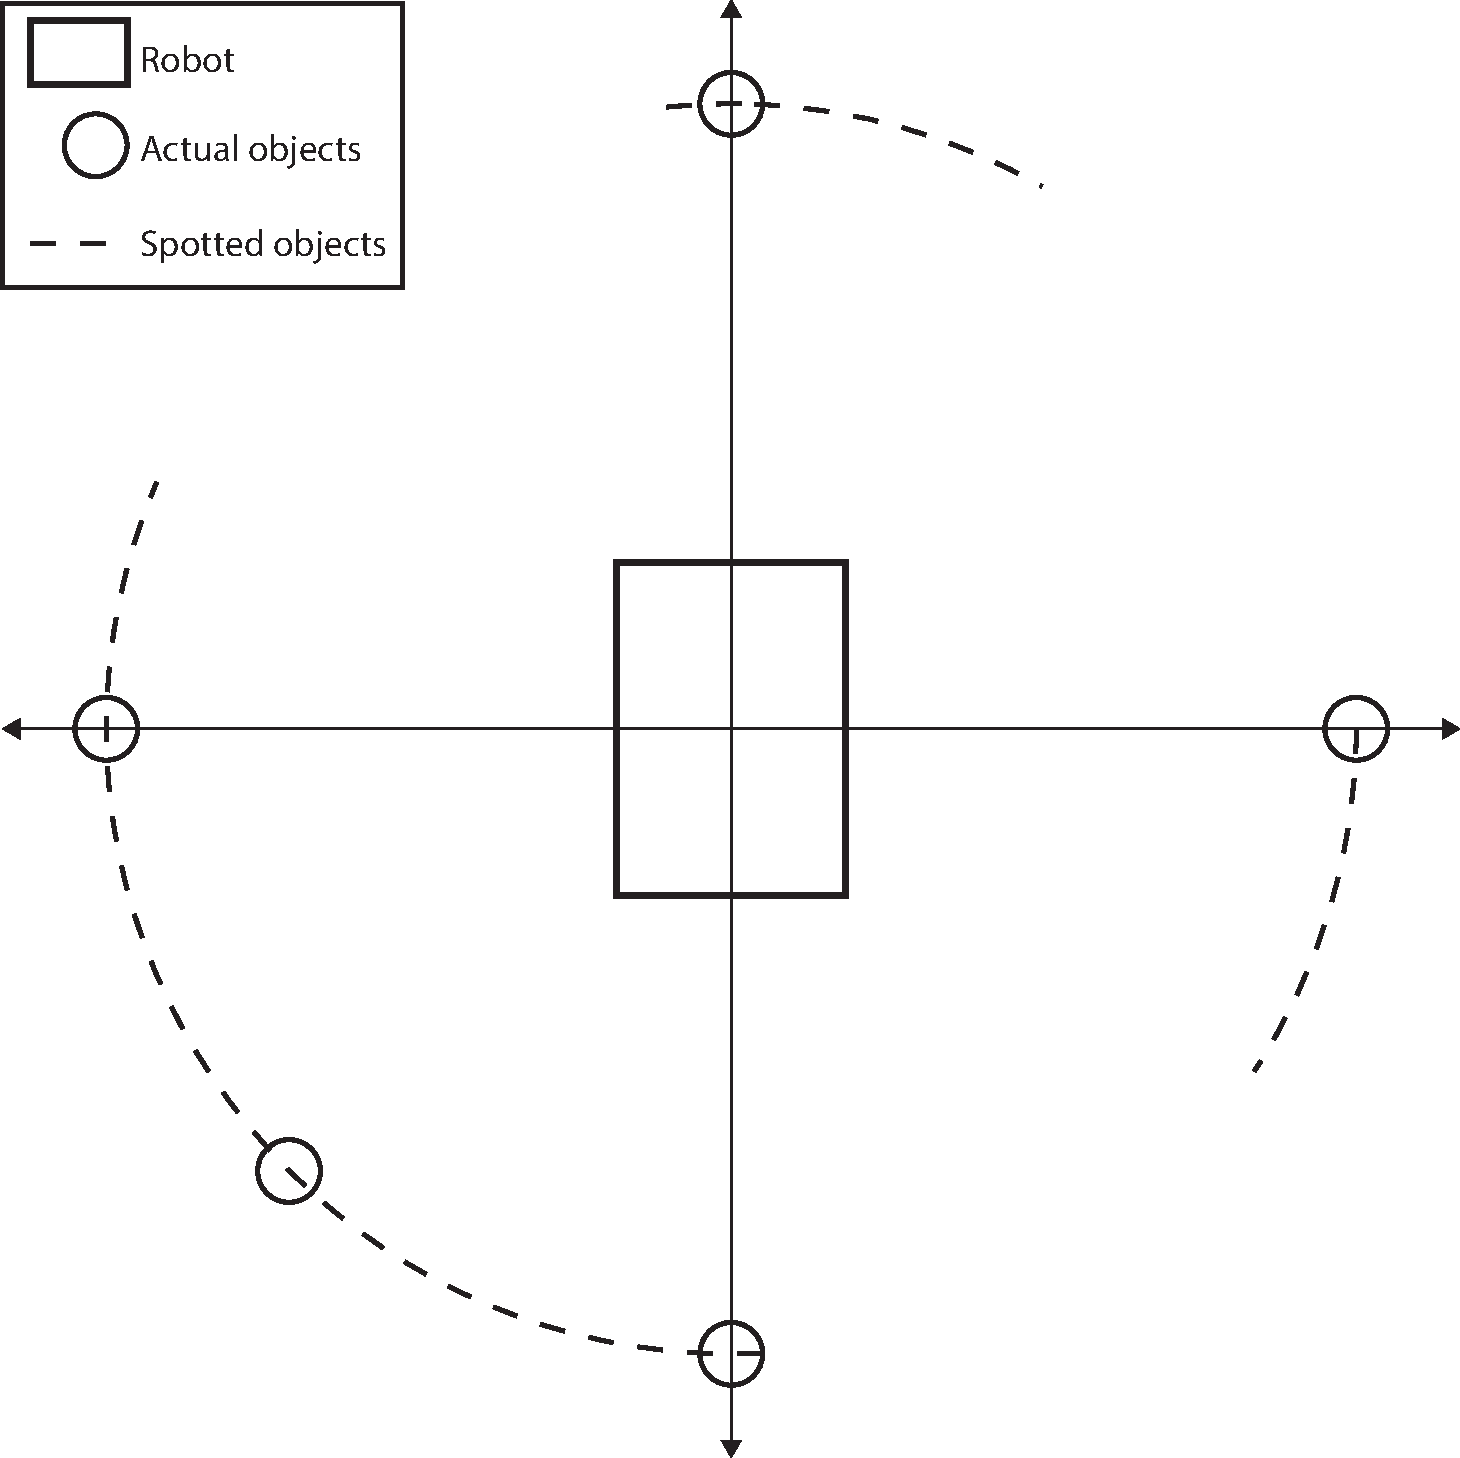
\includegraphics[width=320pt]
     {graphics/SonarTest.pdf}}
     \caption{\label{fig:sonar-test-drawing} 360 degree test with ultrasonic sensor. Graph can be seen in \appref{app:sonar-test-graph}.}
\end{figure}

Last but not least the ultrasonic sensor is having trouble spotting multiple objects if they are standing too close, as seen on the last three objects on \figref{fig:sonar-test-drawing}. It is a matter of the cone being too wide and the first object not being out of sight before the next one is spotted. This results in only one object being added to the object array which means that the \projname{} will get into trouble once it starts collecting.\\
Sometimes the robot is encountering the opposite problem, because sometimes the sound waves does not return despite targeting an object. This break in incoming waves will result in the robot thinking that this is a new object and it will therefore add the same object again.

\subsubsection{Colour sensor} \label{sec:colour_sensor} 
The colour sensor can, by sending out light, measure the reflected light that returns to the sensor. The sensor now contains some raw RGB values, which it can provide the users, or use the integrated colour detecting mechanism to decide which colour it has observed~\citep{lego_education}. 

The test was performed to test the colour sensors ability to detect the black colour which is used as the environment boundary. The sensor should be placed close to the ground, as the only task is to detect the boundary. It should be possible to see a clear difference between the black boundary and the floor. The minimum and maximum values of the black boundary needs to be detected so that \projname{} can distinguish between the floor and the black boundary. Each sensor is tested, where the test provided their respective min and max values after 500 tries. In the end the absolute smallest and largest value is used for each RBG value. This was performed on the boundary and the floor to see the difference between these. A test was also performed, when passing over the black boundary to get the respective values and compare these to the min and max values from the previous test.

\begin{figure}[H]
     \center{\includegraphics[width=\textwidth]
     {graphics/ColorLeft.png}}
     \caption{\label{fig:colour_sensor_test_left} Graph showing RGB values passing the black boundary 12 times for the left colour sensor.}
\end{figure}

\begin{figure}[H]
     \center{\includegraphics[width=\textwidth]
     {graphics/ColorRight.png}}
     \caption{\label{fig:colour_sensor_test_right} Graph showing RGB values passing the black boundary 12 times for the right colour sensor.}
\end{figure}

As seen on \figref{fig:colour_sensor_test_left} and \figref{fig:colour_sensor_test_right}, the two sensors are quite different when it comes to the values they provide, despite being tested the exact same way. This is important and must be taken into account when using the sensors in the program. Due to uncertainties from the environment such as light, shadows, or dust, even the values in the two figures aren't always accurate. To counter this, it is possible to increase the range between the black minimum and maximum detection values to reduce potential detection problems. This increased range is possible, because the floor RGB values compared with the black values are quite different, allowing the addition of this \emph{extended range}.

\begin{table}[H]
	\centering
	\ra{1.3}
	\rowcolors{3}{Gray}{}
    \begin{tabular}{|l|r|r|r|r|r|r|r|r|}
    \hline
    \rowcolor{DGray}
    \textbf{Sensor} & \multicolumn{4}{c|}{Right} & \multicolumn{4}{c|}{Left} \\ \hline
    \rowcolor{Gray}
    \textbf{Surface} & \multicolumn{2}{c|}{Black boundary} & \multicolumn{2}{c|}{Floor} & \multicolumn{2}{c|}{Black boundary} & \multicolumn{2}{c|}{Floor}   \\ \hline
    \rowcolor{DGray}
    \textbf{Colour range}  & Min~~~~ & Max~~~ & Min~~~ & Max~~~ & Min~~~~ & Max~~~ & Min~~~ & Max~~~ \\ \hline
\multicolumn{1}{|l|}{Red}  & 187     & 260    & 329    & 334    & 209     & 282    & 349    & 354    \\ \hline
\multicolumn{1}{|l|}{Green}& 127     & 192    & 252    & 256    & 173     & 253    & 327    & 332    \\ \hline
\multicolumn{1}{|l|}{Blue} & 147     & 198    & 242    & 248    & 182     & 240    & 292    & 297    \\
    \hline
    \end{tabular}
    \caption{\label{table:colour_sensor_test} Colour sensor results on the black boundary and the floor.}
\end{table}

In~\tblref{table:colour_sensor_test}, the min and max values for each sensor is listed. The values reflect the data on \figref{fig:colour_sensor_test_left} and \figref{fig:colour_sensor_test_right}. These values provide the base line for the RGB value range.

It can happen that the \projname{} will drive over the boundary. This happens when the robot drives over it in between two updates from the colour sensor, which is only able to ping a certain amount of times each second. The occurrence of this happening also depends on the width of the boundary.

\subsubsection{Compass sensor}
The HiTechnic NXT Compass Sensor is a digital compass that measures the earth's magnetic field and returns a value representing the current heading. The magnetic heading is calculated to the nearest $1^\circ$ and returned as a number from 0 to 359, where 0 is north and 180 is south~\citep{compass}.

The test of the compass sensor is performed the following way: First the sensor is calibrated to work optimally with the \projname{}. The NXT bricks and the motors on the robot have their own magnetic fields which are noise to the compass sensors readings. This makes sensor calibration prior to use a necessity for accurate output values. The compass sensor will furthermore be placed at least 15cm from the motors and 10cm from the NXT bricks~\citep{compass}.

After the initial calibration the robot is placed facing in a direction close to north, which means a heading of around $0^\circ$. The robot then performs a $720^\circ$ spin while the heading is being logged. Turning clockwise the returned value should be a linear increasing value from 0 and up, until 0 degrees is hit again when the robot is facing north. Turning counter-clockwise, the returned value should quickly jump to $359^\circ$ and linearly decrease while spinning, until north is found again. This will repeat for every $360^\circ$ the robot does.

\begin{figure}[H]
     \center{\includegraphics[scale=1]
     {graphics/DegreesGraph.png}}
     \caption{\label{fig:compass_sensor_test_graph} The measured degrees from a $720^\circ$ counter clockwise turn.}
\end{figure}

\figref{fig:compass_sensor_test_graph} shows the result of a test, where the robot is turning counter-clockwise. The graph illustrates that the compass sensor is outputting the expected values, and thus works as intended. 

\subsubsection{Interactive servo motor} \label{sec:servo_motor}
The LEGO NXT interactive servo motor provides the users movement. The motors have built-in reduction gear assemblies with internal rotation sensors, that measures speed and distance and reports it back to the NXT Brick. This allows for a more precise motor control and the ability to run the motor in steps with one degree of accuracy~\citep{lego_education}.

As the \projname{} has to be able to move around and pick up objects, it would be suitable to drive in a straight line if need be. Therefore the servo motors have been tested to get an idea of a possible difference in performance. The test was set to run for 10 seconds on each motor and measure the degrees of rotation on the specified motor. It was also conducted at different power levels, as the accuracy could vary, depending on the speed. 

\begin{table}[H]
	\centering
	\ra{1.3}
	\rowcolors{1}{Gray}{}
    \begin{tabular}{lccc}
    \hline  
    \rowcolor{DGray}
    \textbf{Power Level}~~~~~~~~~~~~ & Motor L(Degrees) & Motor R(Degrees) & Difference \\ \hline 
    100\%                  & 6,658                  & 6,666                & 0,12\% \\
    90\%                   & 5,823                  & 5,912                & 1,51\% \\
    80\%                   & 5,192                  & 5,262                & 1,33\% \\
    70\%                   & 4,495                  & 4,571                & 1,67\% \\
    60\%                   & 3,859                  & 3,923                & 1,64\% \\
    50\%                   & 3,145                  & 3,211                & 2,07\% \\
    40\%                   & 2,479                  & 2,551                & 2,86\% \\
    \hline 
    \end{tabular}
    \caption{\label{table:servo_motor_test} Servo motor test of rotations.}
\end{table}

As \tblref{table:servo_motor_test} shows, at higher power levels the difference is the smallest, compared to the lower power level, where the difference is increased. This will have an impact on the movement and precision of the \projname{}, therefore this have to be taken into account and adjusted when developing. 

\subsubsection{Object specification} \label{sec:object_specification}
The main task of the \projname{} is to collect objects. Since the \projname{} is considered a prototype, there are restrictions on the objects it is able to pick up. The size of the robot, the strength of the motors and the positions the objects, all presents some limitations on what objects that can be collected by the \projname{}. The different considerations regarding the objects' attributes are:

\begin{itemize}
\item Size - Can the claw get a hold on the object - and detect it? %: height and width.
\item Weight - Can the motors lift the object? %: light and heavy.
\item Shape - Can it hold the object and not let go? %: square and round.
\item Angle - Can the ultrasonic sensor detect the object from all angles? %: 45 degrees and 90 degrees.
\end{itemize}

The size of an objects is important. It is possible to detect objects of 1cm in width, if the object is placed exactly in the middle of the ultrasonic sensor. If the object is over 12cm in width, the claw to collect the object faces complications with the width of the claw. As the robot have to get close to an object to collect it, the width of the ultrasonic sensor can provide a reasonable measurement of the size it should be able to see. If the object is big enough to cover both the sender and receiver, it should be detected. The width is 5cm and given the position of the claw, square objects of size 6x6x6cm, or cylinder objects with a diameter of 6-7cm are preferred.

Different weight of objects have been tested for the robots strength. The robots limit is around 150-200g depending on the object's surfaces friction. If an object is soft and the claw is able to squeeze it, the friction is higher and then the claw is more likely to lift it. It does not matter if the object weight is close to 0g, although the robot tend to push around the objects while trying to grab and if the object is too light there is a chance that it might tip over.

The shape of the object is important; if for instance an object is placed in a way where the ultrasonic sensors sound waves are not immediately reflected back to the sensor, incorrect values will be provided. Square objects with a sharp corner, are hard to detect and constitute a serious problem to the \projname{}. This is described in \secref{sec:ultrasonic_sensor}. 

If an object is a cylinder, the surface of the object is round, meaning the sound waves are always reflected the same way, no matter how it's angled. This means that it will either always be hard, or always be easy, finding cylinder objects, since the angle is irrelevant. This has been tested with different kinds of cans and the robot was always able to detect the cans and always returned proper values. This is unfortunately not good enough for the final non-prototype of the \projname{}, but for the prototype in this project it will be enough. Possible solutions for this can be found in \secref{sec:future_works}.


%When testing how the ultrasonic sensor works with a square object from different angles. If a corner, meaning 45 degrees, is showed towards the sensor, it will deflect the sound waves and not return these, resulting in invalid or disturbed values. The closer to a 90 degrees angle, the more precise it is. ----Det her er udkommenteret da det er beskrevet.


%Based on the documentation the sensor work in the interval from 0 to 2.5 meters and the sensor precision is +/- 3 cm~\citep{lego_edu_guide}. 

%These results show that it is almost staying within boundary of its specifications. There is on the other hand an issue with distances over 150 cm, which it shows at the max of 255 cm.

%At each power level, the test was conducted 3 times per motor and the average was calculated. \fxnote{Testen er ændret til 10sec, som er rettet, men den er kun testet 1 gang per motor ved de forskellige power level, så vi udregner ikke average mere.} 

%As seen from the values in~\tblref{table:colour_sensor_test}, the two sensors are quite different when it comes to their the values they provide. This is a important and must be taken into account when using the sensors in programs. Furthermore, these values are from a stationary source, where as the \projname{} only sees these while driving. This could be a problem. It is observed that the floor- and tape-values are quite different. This means that the boundary of when the \projname{} sees black tape, can be increased, without the \projname{} thinking that it sees the floor. This corrects the issue, and makes sure that the \projname{} detects the black tape. 

%\subsection{Sensors} \label{sec:sensors}
%Forklaring af sensorer og deres funktionalitet.
%(KILDE: LEGO NXT userguide US)
% http://en.wikipedia.org/wiki/Lego_Mindstorms_NXT_2.0

%The touch sensor is a switch which can either be pressed or released. When pressed it gives an output of 1, and when released an output of 0. These states can be used to initiate different actions. 

%The sound sensor is able to detect the decibel level, meaning the softness or loudness of a sound. The sound sensor detects both dB and dBA. dBA is the sounds human ears are able to hear, while dB is all actual sound, including too low or high sounds frequencies for the human ear to hear. The sounds are displayed in percentages, used for comparison.

%The compass sensor is a digital compass, which measures the magnetic field of the earth. It produces an output ranging from 0 to 359 and updates the heading 100 times a second. The compass sensor operates in two modes, read mode and calibrate mode. In calibrate mode, it will compensate for magnetic disturbances.

%The accelerometer sensor lets the LEGO NXT know which way is up when it tilts either up or down, side to side and left or right. It also measures acceleration impact suffered from all sides. 

%The RFID sensor is a radio frequency identification sensor, which consist of two radio frequency transponders. It allows the LEGO NXT to detect and recognise the transponder and triggering a specific behaviour programmed beforehand.

%The rotation sensor(Built in the servo motor) 

%The ultrasonic sensor had a problem when it went beyond 150cm, as seen on \tblref{table:ultrasonic_sensor_test}, the 200cm distance reached max of 255cm. The shortest distance at 10cm, showed that the ultrasonic sensor is imprecise at short distances. Although the test results of the other distances are within decent range of the actual distance, the placement of the ultrasonic sensor could be off by 1cm.\fxnote{Kan vi skrive at den godt kan være "off" med 1cm hvor den blev placeret på gulvet ud fra målingen? NEJ FORHELVEDE. Vi siger jo direkte at vi er idioter til at sætte en ting på jorden.}

% Basic kits udkommenteret:

%\begin{table}[H]
%	\centering
%	\ra{1.3}
%	\rowcolors{1}{Gray}{}
%    \begin{tabular}{lcc}
%    \hline  
%    \rowcolor{DGray}
%    \textbf{Colour}~~~~~~~~~~~~ & Value at approx one stud  & Value at approx two studs \\ \hline 
%    Lowest red                  & 159                      &  \\
%    Lowest green                & 128                      &  \\
%    Lowest blue                 & 132                      &  \\
%    Highest red                 & 188                      &  \\
%    Highest green               & 152                      &  \\
%    Highest blue                & 160                      &  \\
%
%    \hline 
%    \end{tabular}
%    \caption{\label{table:colour_sensor_test} Colour Sensor test RGB-values.}
%\end{table}

%\subsubsection*{Basic kit}
%The basic sensor kit includes a range of different sensors, including a touch sensor, a colour sensor and an ultrasonic sensor. 

%\subsubsection*{Extra sensors}
%Besides the basic kit there exist a number of other sensors that can be used.

